\documentclass[11pt, oneside]{article} 	% use "amsart" instead of "article" for AMSLaTeX format
\usepackage{geometry} 		% See geometry.pdf to learn the layout options. There are lots.
\geometry{letterpaper} 		% ... or a4paper or a5paper or ... 
\usepackage[parfill]{parskip} 		% Activate to begin paragraphs with an empty line rather than an indent
\usepackage{graphicx}				% Use pdf, png, jpg, or eps§ with pdflatex; use eps in DVI mode
								% TeX will automatically convert eps --> pdf in pdflatex		
\usepackage{amssymb}
\usepackage{amsmath}
\usepackage{amsthm}
\usepackage{authblk}
\usepackage{framed}
\usepackage[
backend=biber,
style=alphabetic,
]{biblatex}
\usepackage{graphicx}
\graphicspath{ {./images/} }
\usepackage{verbatim}
\usepackage{tikz} 
\usepackage{subcaption}
\captionsetup{compatibility=false}



\usepackage{tikz}
\usetikzlibrary{positioning, arrows.meta, decorations.pathreplacing}
\usepackage{algorithm}
\usepackage{algpseudocode}
\usepackage{syntonly}
\usepackage{mathabx}
\usepackage{xcolor,colortbl}
\usepackage{framed}



% \syntaxonly \langle -- use this for checking syntax only
% \mbox {text} - keep together
% \fbox {text} - keep together and draw around

%\pagestyle{plain|headings|empty} % header and footer p.27
%SetFonts
%\include{filename}, \includeonly{filename1, filename2} , \input[fiename}

%SetFonts% 


\newtheorem{theorem}{Theorem}[section]
\newtheorem{lemma}[theorem]{Lemma}
\newtheorem{corollary}[theorem]{Corollary}
\newtheorem{proposition}[theorem]{Proposition}
\newtheorem{definition}[theorem]{Definition}

\title{BADG 2: A Perfect Game}
\author{Dave Fetterman}
\date{\today}

\begin{document}

\maketitle

\begin{abstract}
An earlier paper (http://fettermania.com/math/bdice.pdf) focused on a near-optimal strategy for maximizing expected value in gameplay for \textit{Bitches: A Dice Game}.  This paper focuses on a different question: what is the probability of playing a perfect game (and is there any subtlety to doing so)?  Using standard recursive calculation, we calculate the probabilities with the out-of-box game setup.  Then we venture into a related question: What's the expected win probability with $n$ standard dice of side count $s$ as $n \rightarrow \infty?$  We give poor bounds, prove convergence, and find surprising results along the way.
\end{abstract}

\section{Introduction and the Commercial Game}

Outside of ideological patron Larry Waldman, the publication of my original b. a. d. g. paper (http://fettermania.com/math/bdice.pdf) received little fanfare from humans.  However, the robots somehow picked up on this and brought it to the attention of Samuel Cox, creator of the game.  After dispensing mild praise about the paper and strong confusion about my interest in it, Mr. Cox suggested another problem. 

Instead of ``how does one play the game with high/maximum expected value?'' (addressed in the first paper), Mr. Cox wondered how often a \textit{perfect game} (one in which the best possible score is achieved at the end) occurs if played optimally.  Though optimal play looks obvious (pick up all your maximum rolls), Mr. Cox has also debated with his class: ``is it always best to pick up all your maximum-roll dice?''   

I took this on and a day or so later, the solution to this particular question surfaced.  As usual, twinkly subproblems appeared along the way, and I left to find a solution to a related problem: \textit{does the probability of a perfect game converge to a positive number as the number of dice increase to infinity?}.

We'll briefly review the game's rules and the solution method for the commercially offered game before diving in to a discovered second quest: asymptotic behavior of infinite dice.  We'll note surprising or interesting findings in \textit{\textbf{bold-italic}}.

\subsection{The Game}

Though the rules to the multi-player game are detailed in the original paper referenced above, we will reformulate this for a solitaire-style perfect game, which follows this pattern:
\begin{enumerate}
\item Begin with 12 standard dice of six sides, along with one eight-, one ten-, and one twelve-sided die.
\item On each turn, roll all remaining dice in play.
\item If there are no dice with a maximum side showing (e.g. a six-sided die showing six pips), you have lost (``busted'').
\item Set aside some number of dice which have achieved their maximum roll.
\item Continue until no dice remain (you have a perfect game) or you have busted out.
\end{enumerate}

The question \textit{``how likely am I to get a perfect score?''} therefore relies on the \textit{strategy} one employs in picking up dice.  

\subsection{Mistake 1: The Strategy Assumption}
\begin{proposition}[Smoke 'em if you got 'em] The best strategy to achieve a perfect game is to always pick up as many dice with maximum face value as the turn allows.\end{proposition}

This proposition is:
\begin{enumerate}
\item Simple
\item Obvious
\item The strategy any reasonable person would employ
\item Initially assumed for the calculations in the next section
\item \textbf{\textit{Mathematically false}}
\end{enumerate}

In the next section, we assume this simple, deterministic strategy in calculating the expected value of any state reachable from the standard b. a. d. g. starting configuration and show where it goes wrong.

\subsection{Solution Method for the Commercial Game}

The following definitions will help us write a program to get our solution for the commercial game:
\begin{itemize}
\item The ``state'' $\vec{s} := [a,b,c,d]$ is how many dice of size 6, 8, 10, and 12 remain, respectively\footnote{We refer to this often as an arbitrarily-sized vector as well}.  We start at $\vec{S} = [12, 1, 1, 1]$.  A perfect game ends at $\vec{s} = \vec{0}$.  A failure to roll any max roll ends the game in an unlisted `losing' state $\varnothing$.
\item The ``probability vector'' $\vec{p} := [1/6, 1/8, 1/10, 1/12]$ is the chance of getting a max roll from each of the dice sizes, again here assumed to be 6, 8, 10, 12.
\item With a win defined as value $1$ ($F(\vec{0}) = F([0,0,0,0]) = 1$) and a loss as value $0$ ($F(\varnothing) = 0$), the ``expected game value'' of any other state $\vec{s}$ is denoted as $F(\vec{s})$.  Said another way, $F(\vec{s})$ is the probability of ending up in winning state $\vec{0}$ from state $\vec{s}$.
\item We call any state $\vec{t} := [t_1,t_2 ... t_z]$  \textit{reachable} from state $\vec{s} := [s_1,s_2 ... s_z]$ if $t_i \leq s_i$ for all $1 \leq i \leq z$, but $\vec{s} \neq \vec{t}$.  More intuitively, if you can start at state $\vec{s}$ and get to state $\vec{t}$ in one roll (and corresponding pickup) of your dice, then $\vec{t}$ is reachable from $\vec{s}$.  This is just any non-bust state ``smaller than'' where you are now.
\end{itemize}

\subsection{Probability Lemmas}
First, let's limit ourselves to a game (or state) with only a single flavor of dice, say $d$-sided, collapsing state vector $\vec{s}$ to a single integer $r$ ($r$ dice of size $d$ left).  Refer to Fig. \ref{fig:dice-transition} for a partial visualization of the states and transitions starting at $r$ dice left of size $d$, with $p := 1/d, q := 1-p$.

\begin{figure}[ht]
    \centering
    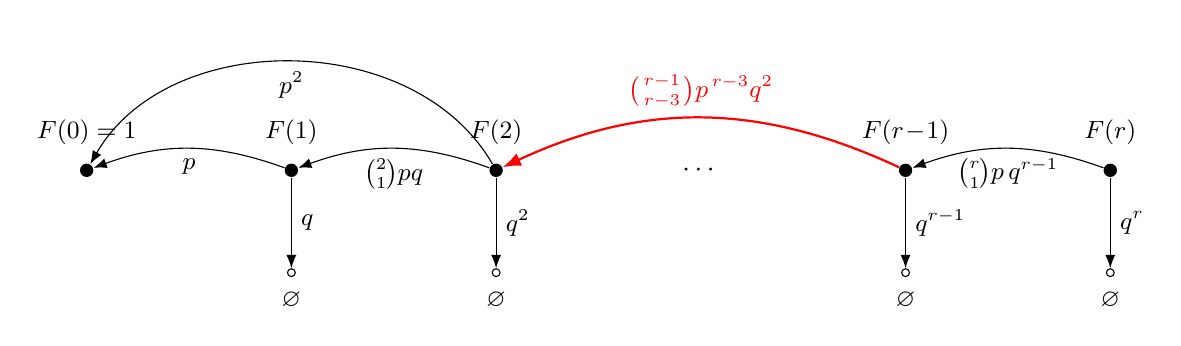
\begin{tikzpicture}[
      >=Latex,
      state/.style={circle,fill=black,inner sep=1.7pt},
      lab/.style={font=\small}
    ]
    
    % positions
    \node[state] (s0) at (0,0)   {};
    \node[state] (s1) at (2.6,0) {};
    \node[state] (s2) at (5.2,0) {};
    \node         (dots) at (7.8,0) {$\cdots$};
    \node[state] (sr1) at (10.4,0) {};
    \node[state] (sr)  at (13.0,0) {};
    
    % labels (top of nodes)
    \node[lab,above=3pt of s0] {$F(0)=1$};
    \node[lab,above=3pt of s1] {$F(1)$};
    \node[lab,above=3pt of s2] {$F(2)$};
    \node[lab,above=3pt of sr1] {$F(r\!-\!1)$};
    \node[lab,above=3pt of sr]  {$F(r)$};
    
    % leftward arrows
    \draw[->] (s1) to[bend right=20] node[lab,below] {$p$} (s0);
    \draw[->] (s2) to[bend right=20] node[lab,below] {$\binom{2}{1}pq$} (s1);
    \draw[->] (s2) to[bend right=60] node[lab,below] {$p^2$} (s0);
    \draw[->] (sr) to[bend right=20] node[lab,below] {$\binom{r}{1}p\,q^{r-1}$} (sr1);
    
    % special red arrow from F(r-1) to F(2)
    \draw[->,red,thick,bend right=25] (sr1) to node[lab,above,sloped,text=red] 
      {$\binom{r-1}{\,r-3\,}p^{\,r-3}q^{2}$} (s2);
    
    % sink/bust nodes
    \node[state,fill=white,draw=black,inner sep=1pt] (z1) at (2.6,-1.3) {};
    \node[state,fill=white,draw=black,inner sep=1pt] (z2) at (5.2,-1.3) {};
    \node[state,fill=white,draw=black,inner sep=1pt] (zr1) at (10.4,-1.3) {};
    \node[state,fill=white,draw=black,inner sep=1pt] (zr) at (13.0,-1.3) {};
    \node[lab,below=2pt of z1] {$\varnothing$};
    \node[lab,below=2pt of z2] {$\varnothing$};
    \node[lab,below=2pt of zr1] {$\varnothing$};
    \node[lab,below=2pt of zr] {$\varnothing$};
    
    % bust arrows with q^t
    \draw[->] (s1) -- node[lab,right] {$q$} (z1);
    \draw[->] (s2) -- node[lab,right] {$q^{2}$} (z2);
    \draw[->] (sr1) -- node[lab,right] {$q^{r-1}$} (zr1);
    \draw[->] (sr) -- node[lab,right] {$q^{r}$} (zr);
    
    \end{tikzpicture}
    \caption{Transition graph of the dice game showing expected values $F(r)$ and transition probabilities.}
    \label{fig:dice-transition}
\end{figure}


\begin{lemma}[EV of $r$ $d$-sided dice]The chance of a completing perfect game from a state of $r$ standard dice of $d$ sides each, with definitions $p := \frac1{d}, P_{single}(r, k, p) := {r \choose k} p^k(1-p)^{r-k},$ and $F(0) = 1$ is defined by the recurrence $F(r) = \sum_{k=1}^r P_{single}(r,k,p) F(r-k)$. \end{lemma}

\textit{Proof}: This a clear application of the binomial theorem.  With the Smoke 'Em if you Got 'Em Strategy, the chance of transitioning to the state with $r-k$ remaining dice from that with $r$ is the chance of rolling exactly $k$ max rolls and $r-k$ non-max rolls among your $d$-sided dice, or $P_{single}(r, k, p)$.  The expected value of being in this new state is defined as $F(r-k)$.  The value of this state transition possibility is $P_{single}(r, k, p)F(r-k)$. The total expected value of being in state $r$ is therefore the sum of the values of all possible state transitions.  Note that $k=0$ implies a roll with no maxes, and thus a loss (value 0), and $F(0) = 1$ since no dice remaining (outside of a loss case) means a victory, or unit value of expectation.

Extending this to dice of $z$ different sizes is clear:

\begin{lemma}[State Transition lemma] $P_{transition}(\vec{s},\vec{t},\vec{p})$, the chance of transitioning from state $\vec{s}=[s_1,s_2,\ldots s_z]$ to state $\vec{t} = [{t}_1, {t}_2\ldots {t}_z]$ with probability vector $\vec{p} = [p_1, p_2 \ldots p_z]$ is equal to
  $\prod_{i=0}^z P_{single}(\vec{s}_i ,\vec{t}_i,\vec{p}_i)$.\end{lemma}


\textit{Proof:} Divide the turn's roll into $z$ independent subrolls, each rolling all $s_i$ dice, $1 \leq i \leq z$, themselves each with $p_i$ chance of hitting a max.  The outcomes of these $z$ subrolls are all mutually independent, so $P_{transition}$ can be expressed as the product of $P_{single}$ quantities.

\subsection{Simple recursive algorithm}

With these easy proofs and definitions in hand, the algorithm follows readily - build up each state from $F(\vec{0})$ to $F(\vec{S})$ by applying the State Transition Lemma and previously computed values of $F$ in Algorithm 1. Notes:
\begin{itemize}
\item Steps 1 - 5 are definitions from the lemmas above.
\item Step 6 creates a set of all states reachable from state $\vec{s}$, \textit{including $\vec{s}$ itself}.  
\item Thinking of the states as a directed graph where a state points to all the states reachable from it, Step 7 creates an ordered list of states $s_1, s_2, s_3...$ , \\
like $[0,0,0,0], [0,0,1,0], [0,1,0,0], [0,1,1,0]....$ where, when $s_i$ is encountered in the list, all states reachable from $s_i$ occur before $s_i$ in the list.  There are many such possible orders. This is required for step 9's $F(\vec{t})$ values to be defined.
\item Step 9 uses Lemma 1.3 to calculate $F(\vec{s})$ from the values of previously calculated substates.
\end{itemize}


\begin{algorithm}[h]
\caption{Dynamic program for $F(\vec{S})$}
\begin{algorithmic}[1]
\State $\vec{S} \gets [12,1,1,1]$
\State $\vec{p} \gets \left[\tfrac{1}{6}, \tfrac{1}{8}, \tfrac{1}{10}, \tfrac{1}{12}\right]$
\State $P_{\text{single}}(r,k,p) := \binom{r}{k} p^k (1-p)^{r-k}$
\State $P_{\text{transition}}(\vec{s_1},\vec{s_2},\vec{p}) := \prod_{i=0}^{\dim(\vec{s})} P_{\text{single}}(\vec{s_1}_i,\vec{s_2}_i,\vec{p}_i)$
\State $F(\vec{0}) \gets 1$
\State $\text{substates}(\vec{s}) := \bigtimes\limits_{i=0}^{dim(s)} [0, s_i] $
\State $\text{states} \gets \text{topological\_sort}\!\left(\text{substates}(\vec{S}) \setminus \{[0,0,0,0]\}\right)$
\For{$\vec{s} \in \text{states}$}
  \State $F(\vec{s}) \gets \sum_{\vec{t} \in \left(\text{substates}(\vec{s}) \setminus \{\vec{s}\}\right)} 
     P_{\text{transition}}(\vec{s},\vec{t}) \cdot F(\vec{t})$
\EndFor
\end{algorithmic}
\end{algorithm}

\subsection{Results for Commercial Game}

Using the Smoke 'Em if you Got 'Em strategy, the chance of winning\footnote{Alternatively, expected value of being in state $F(\vec{s})$, with $F(\vec{0}) = 1, F(\varnothing) = 0$} $F(\vec{s})$ for every state $\vec{s}$, with $\vec{s}$ ranging from $\vec{0}$ to $\vec{S} = [12, 1, 1, 1]$ is listed in Figures \ref{fig:ev-tables-1} and \ref{fig:ev-tables-2}.  These are computed with a simple python program\footnote{https://github.com/fettermania/mathnotes/blob/main/bdice2/bdice2.py}.

Note that this state table is \textit{four-dimensional}, with each dimension $i$ corresponding to the count of dice $s_i$ in each state.  Since the number of 8-, 10-, and 12-sided dice is either zero or one, we've collapsed these into four 12 by 2 tables, where $d_k$ notes the number of dice of size $k$.  

Our main \textit{initial} result for $F(\vec{S})$ is in the bottom-right corner of Fig. \ref{fig:ev-tables-2}.

% First pair of tables
\begin{figure}[ht]
    \centering
    % left table
    \begin{minipage}{0.45\textwidth}
    \centering
    \[
    \begin{array}{c|cc}
    d_6 \backslash d_8 & 0 & 1\\\hline
    0&1&0.125\\
    1&0.1667&0.05642\\
    2&0.07407&0.03244\\
    3&0.04192&0.02206\\
    4&0.02809&0.01679\\
    5&0.02107&0.01378\\
    6&0.01708&0.01195\\
    7&0.01463&0.01076\\
    8&0.01303&0.009966\\
    9&0.01195&0.009423\\
    10&0.01119&0.009044\\
    11&0.01065&0.008779\\
    12&0.01025&0.008591\\
    \end{array}
    \]
    \end{minipage}
    \hfill
    % right table
    \begin{minipage}{0.45\textwidth}
    \centering
    \[
    \begin{array}{c|cc}
    d_6 \backslash d_8 & 0 & 1\\\hline
    0&0.1&0.03469\\
    1&0.04556&0.02046\\
    2&0.02644&0.01425\\
    3&0.01815&0.01109\\
    4&0.01392&0.009299\\
    5&0.01152&0.008218\\
    6&0.01006&0.007537\\
    7&0.009124&0.0071\\
    8&0.008506&0.006818\\
    9&0.00809&0.006638\\
    10&0.007809&0.006529\\
    11&0.007618&0.006468\\
    12&0.007491&0.006441\\
    \end{array}
    \]
    \end{minipage}
    \caption{Expected values for $(d_{10},d_{12})=(0,0)$ (left) and $(1,0)$ (right).}
    \label{fig:ev-tables-1}
\end{figure}

% Second pair of tables
\begin{figure}[ht]
    \centering
    % left table
    \begin{minipage}{0.45\textwidth}
    \centering
    \[
    \begin{array}{c|cc}
    d_6 \backslash d_8 & 0 & 1\\\hline
    0&0.08333&0.02908\\
    1&0.03819&0.01726\\
    2&0.02231&0.01209\\
    3&0.0154&0.009464\\
    4&0.01188&0.00798\\
    5&0.009888&0.007088\\
    6&0.008677&0.006532\\
    7&0.007907&0.006181\\
    8&0.007404&0.00596\\
    9&0.007071&0.005825\\
    10&0.006851&0.00575\\
    11&0.006707&0.005715\\
    12&0.006618&0.005709\\
    \end{array}
    \]
    \end{minipage}
    \hfill
    % right table
    \begin{minipage}{0.45\textwidth}
    \centering
    \[
    \begin{array}{c|cc}
    d_6 \backslash d_8 & 0 & 1\\\hline
    0&0.02347&0.01087\\
    1&0.01406&0.007809\\
    2&0.009946&0.006252\\
    3&0.007849&0.005385\\
    4&0.006672&0.004879\\
    5&0.005971&0.00458\\
    6&0.005542&0.004408\\
    7&0.005278&0.004318\\
    8&0.00512&0.004283\\
    9&0.005033&\cellcolor{yellow}0.004284\\
    10&0.004994&0.004312\\
    11&0.004988&0.004356\\
    12&\cellcolor{yellow}0.005005&0.004413\\
    \end{array}
    \]
    \end{minipage}
    \caption{Expected values for $(d_{10},d_{12})=(0,1)$ (left) and $(1,1)$ (right).}
    \label{fig:ev-tables-2}
\end{figure}

\subsection{Observations}
Observations from Figs. \ref{fig:ev-tables-1} and \ref{fig:ev-tables-2}:
\begin{itemize}
\item Most of the time, starting with some state $\vec{s}$ and picking up one or more dice will increase the expected value of winning.
\item However, we do note some non-monotonicity: there are two surprising ``critical points'' at $[12,0,1,1]$ and $[9, 1, 1, 1]$, where instead of the EV decreasing as $d_6$ increases, the EV increases instead.  This means that, for example, the best strategy when rolling two max-sixes and no other max dice in state $[10, 1, 1, 1]$ is to \textit{\textbf{leave one max die on the table}} so as to end up in slightly higher EV state $[9,1,1,1]$ over $[8,1,1,1]$.  We will revisit these in the next section.
\item At all states reachable from $[12, 0, 1, 1]$, the best strategy is confirmed: pick up as many max-rolled dice as possible.  Deviating from this strategy produces an $F$-value smaller than those in the table. \textit{Note:} The ``bend'' at $[11,0,1,1]$ does not affect this; you have no alternative from [12,0,1,1] than to pick up if [11,0,1,1] if you roll one max-six.
\item At all states reachable from $[10,1,1,1]$, the simple strategy remains best.
\item We can confirm that holding $d_6$ steady, it's always better to have zero than one of each of the 8, 10, and 12-sided dice.
\end{itemize}

\begin{framed}
\textbf{What The Creator Asked For}: The chance of getting a perfect run the commercial game using the Smoke 'Em strategy is about 0.004413, or a little more than 4.4\%.
\end{framed}

\subsection{Re-examining The optimal strategy}

From examining the table it becomes clear that there are expected values for states $\vec{s}, \vec{t}$ such that $\vec{t}$ is reachable from $\vec{s}$ yet $F(\vec{t} ) < F(\vec{s})$.  

This means we need to refine our formula to choose the best selectable EV state from state $\vec{s}$, not just the furthest from $\vec{s}$.  With this definition in hand:

$selectable\_states(\vec{s}, \vec{t}) := (substates(\vec{s}) - \vec{s}) - substates(\vec{t}) + \vec{t}$

update Step 9 of Algorithm 1 above to: 

$F(\vec{s}) \gets \sum_{\vec{t} \in \left(\text{substates}(\vec{s}) - \{\vec{s}\}\right)} 
     P_{\text{transition}}(\vec{s},\vec{t}) \cdot max_{\vec{u} \in selectable\_states(\vec{s}, \vec{t})} F(\vec{u})$
     

Because F monotonically decreases as all of $d_6, d_8, d_{10}, d_{12}$ increase up to these critical points, these two functions will be equal on states reachable from $[10,1,1,1]$ and $[12,0,1,1]$.

We then need to recursively reevaluate $F$ on ``bigger'' states than $[9,1,1,1]$, shown in Fig. \ref{fig:ev-tables-corrected}.

\begin{figure}[ht]
    \centering
    \[
  \begin{array}{c|cc}
  d_6 \backslash d_8 & 0 & 1\\\hline
  0&0.02347&0.01087\\
  1&0.01406&0.007809\\
  2&0.009946&0.006252\\
  3&0.007849&0.005385\\
  4&0.006672&0.004879\\
  5&0.005971&0.00458\\
  6&0.005542&0.004408\\
  7&0.005278&0.004318\\
  8&0.00512&0.004283\\
  9&0.005033&0.004284\\
  10&0.004994&\cellcolor{pink}0.004312 \rightarrow 0.004312\\
  11&0.004988&\cellcolor{pink}0.004356 \rightarrow 0.004366\\
  12&0.005005&\cellcolor{pink}0.004413 \rightarrow0.004446\\
  \end{array}
    \]
    \caption{Expected values for $(d_{10},d_{12})=(0,1)$ (left) and $(1,1)$ (right).}
    \label{fig:ev-tables-corrected}
\end{figure}


\begin{framed}
\textbf{What The Creator Really Asked For}: The chance of getting a perfect run the commercial game using the very best strategy (smoke 'em except leave a second and final unsupported six on $[d_6 \in \{10,11,12\},d_8=1,d_{10}=1,d_{12}=1]$) is about 0.004446, or a little more than 4.4\%, a 0.73\% relative improvement on the smoke 'em strategy.
\end{framed}

So it turns out Mr. Cox's students are correct - you may indeed want to ``save'' future six rolls if your rarer ``onesies'' remain.  The difference on the commercial game begins at $[10,1,1,1]$, and occurs exactly when you roll exactly 2 sixes on 6-sided dice and no other maxes.

\begin{itemize}
 \item $[10,1,1,1]$: Naive: Take both sixes (EV = 0.0043116537).  \textbf{Optimal}: Take only 1 six (EV = 0.0043120029).
 \item $[11,1,1,1]$: Naive: Take both sixes (EV = 0.0043564817).  \textbf{Optimal}: Take only 1 six (EV = 0.0043662025).
 \item $[12,1,1,1]$: Naive: Take both sixes (EV = 0.0044132805).  \textbf{Optimal}: Take only 1 six (EV = 0.0044456381).
\end{itemize}

It's nice to see the game is complex and non monotonic even in this constrained scenario.    There are likely higher configurations yielding other critical points in the space, especially as more dimensions (dice types) are added.  Though the difference is minuscule in the commercial game, expanding $\vec{S}$ to something like $\vec{S^*} = [24,2,2,2]$ yields a wider EV difference between simple and optimal strategies\footnote{$F(\vec{S^*}) = 0.0033078600$ using the basic strategy and $0.0038614244$ using the optimal, a 17\% improvement}.

\section{The Second Quest: $d_6 \rightarrow \infty$}

But can we say nothing more definitive than that?  Looking at the left column on the first table (Fig. \ref{fig:ev-tables-1}) with only one type of die, it looks like a higher dice count both decreases our chance of winning, but may also do so asymptotically.

Let's run $\vec{S} = [r, 0, 0, 0], r \rightarrow \infty$ and see (Table \ref{tab:p_values}).


\begin{table}[h]
\centering
\begin{tabular}{|c|c|}
\hline
$r$ & $F(r)$ \\
\hline
0 & 1.000000000000000 \\
1 & 0.166666666666667 \\
2 & 0.074074074074074 \\
3 & 0.041923868312757 \\
4 & 0.028091341512981 \\
5 & 0.021074519393544 \\
6 & 0.017084426737672 \\
7 & 0.014629278661270 \\
8 & 0.013031406311202 \\
9 & 0.011947904221376 \\
10 & 0.011190349681739 \\
\hline
\vdots & \vdots \\
\hline
90 & 0.009033527660227 \\
91 & 0.009033527656758 \\
92 & 0.009033527653985 \\
93 & 0.009033527651768 \\
94 & 0.009033527649995 \\
95 & 0.009033527648578 \\
96 & 0.009033527647444 \\
97 & 0.009033527646538 \\
98 & 0.009033527645813 \\
99 & 0.009033527645234 \\
100 & 0.009033527644770 \\
\hline
\end{tabular}
\caption{Values of $F(r)$ with $p=\frac1{6}$}
\label{tab:p_values}
\end{table}


It certainly looks like there is an asymptote to which $F(\vec{s})$ converges.  This will be the thrust of the rest of this paper: examining the infinite game of $F(\vec{s})$ with one type of die.  \textbf{But can we prove there is an asymptote?}

Two notes:

\begin{itemize}
\item We only have one type of die now, and if we have $r$ of them left, the EV of that state is given as $F(r)$ (we changed $F$ to take integers now instead of vectors).
\item  Unless we see an inflection point ($F(r)$ reverses direction and starts \textit{increasing} past a certain point), the simple strategy and optimal strategy (from section 1) are equivalent.  
\item If we can find $\lim_{r \rightarrow \infty} F_d(r), $ with dice of size $d$ and $\lim_{r \rightarrow \infty} F_g(r)$ with dice of size $g > d$, then it's clear that an infinite proportional \textit{mix} of these dice will fall between them; this is not examined further.
\end{itemize}

\subsection{Mathematical Lemmas}

\textit{Note: For some $d$-sided die, we assume $p := 1/d, q := 1-p$ for the rest of the paper.}

To restate $F$ for a single die value:

\begin{definition}[EV of Game at state $r$]The expected value of the game with $r$ fixed $d$-sided dice is 1 at $r = 0$, and when $r > 0$, is defined by $F(r) = \sum_{k = 1}^r {r \choose k}p^kq^{r-k} F(r-k)$.\end{definition}

\begin{lemma}[Easy Cases Lemma] If $p = 0$, F(r) = 0.  If $p = 1, F(r) = 1$. If $p = \frac1{2}$, for any $r > 0,F(r) = \frac{1}{2}$.
\end{lemma}
\textit{Proof}: 
Though we won't be flipping infinite $(p=0)$ or 1-sided $(p=1)$, dice, these algebraic identities are obvious (can't succeed, can't fail, respectively) and will be useful later.

\textbf{Base case for $p=\frac1{2}$}: $F(1) = \frac1{2}$ since a perfect game occurs if and only if the 2-die (coin, really) shows 2 instead of 1.

\textbf{Inductive case for $p=\frac1{2}$}: Assuming $F(k) = \frac1{2}$ for all $0 < k < r$,  and $F(0) = 1$:
\begin{align*}
F(r) &= \sum_{k=1}^{r-1} {r \choose k} p^k q^{r-k} F(r-k) + {r \choose r} p^r q^0 F(0) \\
&= [ {r \choose 1}  +  {r \choose 2 } + \ldots +  {r \choose r-1}] \frac1{2^r} (\frac1{2}) + \frac1{2^r} 2(\frac1{2}) \\
&= (2^r - 2) \frac1{2^r} (\frac1{2}) + 2\frac1{2^r} (\frac1{2}) \\
&= (2^r) \frac1{2^r} (\frac1{2})\\
&=  \frac1{2}
\end{align*}

For simplicity, we consider only $p \leq \frac1{2}$ from here on out\footnote{Swap ``$q$'' for ``$p$'' in all statements if $p > \frac1{2}$ and you'll find mirrored results (e.g. $p$ converges upward)}. 

\begin{lemma}[Lazy Upper Bound for $F(r)$] With $r \geq 1$ dice left and $F(r) \leq p$.
\end{lemma}
\textit{Proof}: See Fig. \ref{fig:dice-transition}.  Any successful path from state $r > 0$ to state $0$ has a final jump of the form $p^k, k \leq r$.  For instance, the ``low'' path in Fig. \ref{fig:dice-transition} would have probability $F(r) = [{r \choose 1}pq^{r-1}] [{r \choose 1}p^{r-3}q^2] [{2 \choose 1}pq] p^1$.  A single, near-miraculous jump from state $r$ would have probability $F(r) = p^r$.  In any case, $F(r) = M(r,p)p^k$ for some $M(r,p) \leq 1$, and some $k \geq 1$ for the final stage before 0.  Since $p^k \leq p$ for $k \geq 1$, $F(r) = M(r,p)p^k < p^k \leq p$.

\begin{lemma}[Lazy Lower Bound for $F(r)$ (Pochhammer form)] With $r \geq 1$ dice remaining, $F(r) \geq \prod_{i=1}^k (1-q^k)$.
\end{lemma}
\textit{Proof}: See Fig. \ref{fig:dice-transition}.  Any successful path passes through a set of these stages $r \ldots 0$ \textit{without once} falling into the state $\varnothing$.  This means that if state $k$ is included in the path, that there was a $(1-q^k)$ chance of not busting at that stage.  So, assuming our successful path visited every single stage (picking up exactly one die each time), the chance of success would be at least $F(r) = \prod_{i=1}^k (1-q^k)$, since we survived every ``bust trap''.  However, we need not visit every stage (we could possibly pick up more than one die).  Therefore, $F(r) \geq \prod_{i=1}^k (1-q^k)$.

Interestingly enough, \textit{\textbf{this lower bound for $F(r)$ is a known quantity called the q-Pochhammer symbol $(q;q)_\infty = \prod_{i=1}^k (1-q^k)$, with known convergence properties,}} appearing in areas like quantum algebra and physics.  News to me.  Neato.

However, this symbol does not have a closed form evaluation.  Let's try to find a closed form bound that's even WORSE than this one.

\begin{lemma}[Closed Form Lower Bound Lemma]For an unbounded set of $r > 0$ dice, $p \leq \frac1{2}$, the probability $F(r)$ of getting a perfect game has a lower bound of $\exp(-\frac{q}{(1-q)^2})$.
\end{lemma}
\textit{Proof}:
\begin{itemize}
\item First we have $F(r) \geq \prod_{k=1}^r (1-q^k)$ from the Lazy Lower Bound lemma.
\item This means $\log(F(r)) \geq \sum_{k=1}^r \log(1-q^k)$ 
\end{itemize}


Often, $\log(1-z)$ is approximated by $-z$ near zero, but we are most concerned with $z$ near one, since $1-z$ approaches 0, and $\log(1-z)$ explodes.  Therefore, let's look at the expansion of $\log(1-z)$:
\begin{itemize}
\item Identity 1: $f(z) = -\frac1{1-z} = - 1 - z - z^2 -  \ldots$
\item Identity 2: $\int f(z) = \log(1-z) = -z-\frac{z^2}{2} - \frac{z^3}{3} - \ldots$
\end{itemize}

So when summing $\sum_{i=1}^k \log(1-q^k)$, we can instead sum:
\begin{align}
\log(F(r)) &= \log(1-q^1) + \log(1-q^2) + \log(1-q^3) + \cdots \\
&= \left(-q - \frac{q^2}{2} - \frac{q^3}{3} - \cdots\right) + \left(-q^2 - \frac{q^4}{2} - \frac{q^6}{3} - \cdots\right) \nonumber \\
&\quad + \left(-q^3 - \frac{q^6}{2} - \frac{q^9}{3} - \cdots\right) + \cdots \\
&> \left(-q - q^2 - q^3 - \cdots\right) + \left(-q^2 - q^4 - q^6 - \cdots\right) \nonumber \\
&\quad + \left(-q^3 - q^6 - q^9 - \cdots\right) + \cdots \\
&= \frac{-q}{1-q} + \frac{-q^2}{1-q^2} + \frac{-q^3}{1-q^3} + \cdots \\
&> \frac{-q}{1-q} + \frac{-q^2}{1-q} + \frac{-q^3}{1-q} + \cdots \\
&= \frac{1}{1-q}\left[-q - q^2 - q^3 - \cdots\right] \\
&= \frac{-q}{(1-q)^2}
\end{align}

\begin{itemize}
\item (2) follows from (1) by substitution using Identity 2 above.
\item (3) follows from (2) since the denominators of (2) are larger.
\item (4) follows from (3) when dividing each sequence by $-q^k$  and applying identity 1.
\item (5) follows from (4) since the denominators of (4) are larger.
\item (6) and (7) follow from (5) by dividing out $\frac1{1-q}$ and applying Identity 2.
\end{itemize}

Since $\log(F(r))  > \frac{-q}{(1-q)^2}$, $F(r) > \exp (\frac{-q}{(1-q)^2})$.

\[
\begin{array}{c|c|c|c}
q & P(\infty) & (q;q)_\infty & \exp\!\left(-\tfrac{q}{(1-q)^2}\right) \\
\hline
1/2  & 5.0000 \times 10^{-1} & 2.8879 \times 10^{-1} & 1.3534 \times 10^{-1} \\
2/3  & 1.9827 \times 10^{-1} & 6.9272 \times 10^{-2} & 2.4788 \times 10^{-3} \\
3/4  & 7.3137 \times 10^{-2} & 1.5545 \times 10^{-2} & 6.1442 \times 10^{-6} \\
4/5  & 2.5997 \times 10^{-2} & 3.3680 \times 10^{-3} & 2.0612 \times 10^{-9} \\
5/6  & 9.0335 \times 10^{-3} & 7.1400 \times 10^{-4} & 9.3576 \times 10^{-14} \\
6/7  & 3.0912 \times 10^{-3} & 1.4913 \times 10^{-4} & 5.7495 \times 10^{-19} \\
7/8  & 1.0461 \times 10^{-3} & 3.0815 \times 10^{-5} & 4.7809 \times 10^{-25} \\
8/9  & 3.5109 \times 10^{-4} & 6.3155 \times 10^{-6} & 5.3802 \times 10^{-32} \\
9/10 & 1.1705 \times 10^{-4} & 1.2861 \times 10^{-6} & 8.1940 \times 10^{-40} \\
\end{array}
\]
This is a very poor bound, especially when compared to $(q;q)_\infty$.   But being able to prove Lemma 2.3 and 2.5 in closed form (or without relying on the Pochhammer result) yields this surprising result:

\begin{corollary}[Bounded Results for $F(r)$ as $r \rightarrow \infty$] As $p \rightarrow 0$, $F(r)$ can be made arbitrarily close to 0.  However, for fixed $p > 0$, $F(r) > \epsilon$ as $r \rightarrow \infty$ for some $\epsilon > 0$.
\end{corollary}
The upshot: \textit{\textbf{Though increasing the number of sides of the dice can drive F(r) to zero, increasing the number of dice (r) to infinity will never drive F(r) below some fixed constant dependent only on $p$.}}

There are a few ways to make this stronger:
\begin{enumerate}
\item Find a closed form solution for $F(r)$.
\item Find a solution for the asymptote of F(r) as $r \rightarrow \infty$.
\item Prove that $F(r)$ actually converges (instead of just ``is bounded'') as $r \rightarrow \infty$.
\end{enumerate}

We will show why (1) is unlikely, that (3) is true, and hope to one day get better bounds for (2) than lemmas 2.3 and 2.5.

\subsection{An Unlikely Closed Form}

Definition 2.1, again is $F(r) = \sum_{k = 1}^r {r \choose k}p^kq^{r-k} F(r-k), r > 0$, with $F(0) = 1$.


Definition 2.1 is a complicated recurrence; each successive $F(r)$ depends not only on the previous result $F(r-1)$ but \textit{all} previous results $F(r-j), 0 \leq j \leq r$.

Applying Definition 2.1 by hand yields:

\textbf{Table A: List of F(r)}:

\[
\begin{aligned}
F(0) &= 1, \\[6pt]
F(1) &= p, \\[6pt]
F(2) &= p^{2}\,\bigl(1 + 2q \bigr), \\[6pt]
F(3) &= p^{3}\,\bigl(1 + 3q + 3q^{2} + 6q^{3} \bigr), \\[6pt]
F(4) &= p^{4}\,\bigl(1 + 4q + 6q^{2} + 16q^{3} + 12q^{4} + 12q^{5} + 24q^{6} \bigr), \\[6pt]
F(5) &= p^{5}\,\bigl(1 + 5q + 10q^{2} + 30q^{3} + 35q^{4} + 50q^{5} + 90q^{6} + 80q^{7} + 60q^{8} + 60q^{9} + 120q^{10} \bigr), \\[6pt]
F(6) &= p^{6}\,\bigl(1 + 6q + 15q^{2} + 50q^{3} + 75q^{4} + 126q^{5} + 240q^{6} + 300q^{7} + 360q^{8} + 390q^{9} \\
&\qquad\qquad\;\; + 660q^{10} + 540q^{11} + 480q^{12} + 360q^{13} + 360q^{14} + 720q^{15} \bigr).
\end{aligned}
\]

This pattern in this form isn't yet obvious.  Let's look at differences $F(r) - F(r+1)$; if these converge or are bounded, we have hope for a closed form solution:

\textbf{Table B: List of F(r) - F(r+1)}:


\[
\begin{aligned}
F(0) - F(1) &= 1 \,\bigl( 1 - p\bigr), \\[6pt]
F(1) - F(2) &= p \,\bigl( 1 - p - 2pq \bigr), \\[6pt]
F(2) - F(3) &= p^{2}\,\bigl( 1 + 2q - p - 3pq - 3pq^{2} - 6pq^{3} \bigr), \\[6pt]
F(3) - F(4) &= p^{3}\,\bigl( 1 + 3q + 3q^{2} + 6q^{3} \\
&\qquad - p - 4pq - 6pq^{2} - 16pq^{3} - 12pq^{4} - 12pq^{5} - 24pq^{6} \bigr), \\[6pt]
F(4) - F(5) &= p^{4}\,\bigl( 1 + 4q + 6q^{2} + 16q^{3} + 12q^{4} + 12q^{5} + 24q^{6} \\
&\qquad - p - 5pq - 10pq^{2} - 30pq^{3} - 35pq^{4} - 50pq^{5} - 90pq^{6} \\
&\qquad - 80pq^{7} - 60pq^{8} - 60pq^{9} - 120pq^{10} \bigr), \\[6pt]
F(5) - F(6) &= p^{5}\,\bigl( 1 + 5q + 10q^{2} + 30q^{3} + 35q^{4} + 50q^{5} + 90q^{6} + 80q^{7} + 60q^{8} + 60q^{9} + 120q^{10} \\
&\qquad - p - 6pq - 15pq^{2} - 50pq^{3} - 75pq^{4} - 126pq^{5} - 240pq^{6} \\
&\qquad - 300pq^{7} - 360pq^{8} - 390pq^{9} - 660pq^{10} - 540pq^{11} \\
&\qquad - 480pq^{12} - 360pq^{13} - 360pq^{14} - 720pq^{15} \bigr).
\end{aligned}
\]


\begin{proposition}[F(r) does not have a closed form] 
\end{proposition}
\textit{Thoughts, not a proof}:
\begin{itemize}
\item Since the degree of $p$ in $F(r)$ is $\frac{r(r+1)}{2}$, this suggests $F$'s successive functions become more complicated than a closed from allows.
\item Lemma 2.2 also shows $F(r) =  \frac1{2}$ when $p = \frac1{2}$ for any $r > 0$.  This means that $F(r+1)-F(r)$ \textit{does} collapse always at $p = \frac1{2}$ (also 0, 1), but must be nonzero at some $p=\frac1{2} - \epsilon$ as well.  

\end{itemize}

Though not a proof, these suggest \textit{\textbf{there may not be a fundamentally simpler way to capture our multi-way recurrence than a polynomial whose leading coefficient is a triangle number in r!}} Then, my next failed attempt to find a solution focused instead on the seemingly monotonic behavior of $F(r), r \rightarrow \infty$ for fixed $p < \frac1{2}$.

\subsection{F(r) is non-monotonic}


\begin{theorem}[Incorrect Blind Alley: $F(r+1) < F(r), r > 0$] If $p < \frac1{2}, F(r+1) < F(r)$ for $r > 0$.\end{theorem}
\textit{Failed Proof}: This certainly seems obvious.  Perhaps there are reformulations or combinatorial identities that allow the reduction of Definition 2.1 to something manageable.

The bugbear of $F(r)(\frac1{2})=\frac1{2}$ made sure, however, that successive differences had to be extremely small near $\frac1{2}$, so no real daylight poked through. Additionally, there are countervailing forces as well: you are \textit{less} likely to fail on stage $r+1$ (immediate bust probability: $q^{r+1}$) than stage $r$ (immediate bust probability: $q^r$), but more likely to land further away from stage 0 than at stage $r$, presumably worse EV by induction.

All hope was lost when the counterexample was found.

\begin{proposition}[Counterexample to Monotonicity]$F(r) < F(r+1)$ for certain values of $r > 0, p < \frac1{2}$.\end{proposition}

Consider that at $p = \frac1{2}, F(r) = F(s) = \frac1{2}$ for any $r, s > 0$, and therefore, $F(r) - F(r+1) = 0$.  If $F(r) > F(r+1)$ when $p < \frac1{2}$, we can know with $p$ at anydistance $\epsilon$ below $\frac1{2}$, that the difference will be positive.
  
First, reformulate each of the expressions in \textbf{Table B} as dependent on this $\epsilon$: with $p \rightarrow \frac1{2} - \epsilon,  q \rightarrow \frac1{2} + \epsilon$:

\textbf{List of F(r) - F(r+1), as a function $\epsilon$}:

\[
\begin{aligned}
F(1) - F(2) &= -2 \epsilon^{3} + \tfrac{1}{2}\,\epsilon, \\[6pt]
F(2) - F(3) &= 6 \epsilon^{6} + 3 \epsilon^{5} - 3 \epsilon^{4} - \tfrac{3}{2}\,\epsilon^{3} + \tfrac{3}{8}\,\epsilon^{2} + \tfrac{3}{16}\,\epsilon, \\[6pt]
F(3) - F(4) &= -24 \epsilon^{10} - 36 \epsilon^{9} + 20 \epsilon^{7} + 11 \epsilon^{6} - \tfrac{5}{2}\,\epsilon^{5} - 4 \epsilon^{4} - \tfrac{1}{4}\,\epsilon^{3} + \tfrac{13}{32}\,\epsilon^{2} + \tfrac{3}{64}\,\epsilon, \\[6pt]
F(4) - F(5) &= 120 \epsilon^{15} + 360 \epsilon^{14} + 330 \epsilon^{13} - 40 \epsilon^{12} - \tfrac{485}{2}\,\epsilon^{11} - \tfrac{267}{2}\,\epsilon^{10} - \tfrac{7}{8}\,\epsilon^{9} + 50 \epsilon^{8} \\
&\quad + \tfrac{925}{32}\,\epsilon^{7} - \tfrac{9}{32}\,\epsilon^{6} - \tfrac{801}{128}\,\epsilon^{5} - \tfrac{71}{32}\,\epsilon^{4} + \tfrac{185}{512}\,\epsilon^{3} + \tfrac{135}{512}\,\epsilon^{2} + \tfrac{3}{2048}\,\epsilon, \\[6pt]
F(5) - F(6) &= -720 \epsilon^{21} - 3600 \epsilon^{20} - 7200 \epsilon^{19} - 6420 \epsilon^{18} - 315 \epsilon^{17} + 4560 \epsilon^{16} + 3810 \epsilon^{15} + 720 \epsilon^{14} \\
&\quad - \tfrac{6285}{8}\,\epsilon^{13} - \tfrac{6205}{8}\,\epsilon^{12} - \tfrac{2893}{8}\,\epsilon^{11} + \tfrac{231}{32}\,\epsilon^{10} + \tfrac{13305}{128}\,\epsilon^{9} + \tfrac{1985}{32}\,\epsilon^{8} \\
&\quad + \tfrac{1387}{128}\,\epsilon^{7} - \tfrac{1273}{128}\,\epsilon^{6} - \tfrac{21449}{4096}\,\epsilon^{5} - \tfrac{1405}{4096}\,\epsilon^{4} + \tfrac{425}{1024}\,\epsilon^{3} \\
&\quad + \tfrac{2047}{16384}\,\epsilon^{2} - \tfrac{423}{65536}\,\epsilon.
\end{aligned}
\]

We're looking to see if F(r) - F(r+1) is ever negative, and we need look no further than $F(5) - F(6)$, for small $\epsilon$.   Notice that if $\epsilon$ is almost zero, the final term in each sum $C\cdot \epsilon$ for some $C$ will dominate the expression, as $\epsilon^2, \epsilon^3...$ will be exceedingly small.  For $F(1) - F(2), F(2) - F(3), F(3) - F(4)$ and $F(4) - F(5)$, the final  $C$ is positive, but for $F(5) - F(6)$, C = $-\frac{423}{65536}$.  This means that for small epsilon, looking at $p = \frac1{2} - \epsilon$ may yield an increase in EV as we move from 5 to 6 dice left.

Sure enough, for $\epsilon = .005, (p = .495)$, we see that $F(r+1)$ can be greater than $F(r)$ in Table  \ref{tab:p_values_epsilon}:


\begin{table}[h]
\centering
\begin{tabular}{|c|c|}
\hline
$r$ & $F(r)$ \\
\hline
0 & 1.000000000000000 \\
1 & 0.495 \\
2 & 0.49250025 \\
3 & 0.49155356436553116 \\
4 & 0.4913090668731703 \\
5 & \cellcolor{yellow}0.4912951070978062 \\
6 & 0.4913242043135742 \\
7 & 0.4913441989090334 \\
8 & \cellcolor{yellow}0.49135032152170444 \\
9 & 0.4913486656274434 \\
10 & 0.4913447466697759 \\
\hline
\end{tabular}
\caption{Values of $F(r)$ with $p=0.495$}
\label{tab:p_values_epsilon}
\end{table}


We can see that $F(r)$ will reverse directions (yellow cells) as $r$ increases, though it does asymptotically approach something like 0.4913417493573063 as $r \rightarrow \infty$.

With monotonicty and bounds, convergence is assured.  Without it, we must show convergence another way.

\subsection{F(r) converges as $r \rightarrow \infty$}

\begin{theorem}[F(r) convergence]: $F(r)$ converges when $p \leq \frac1{2}$.\end{theorem}

Notice that each term $F(k)$ in table A is of the form $F(k) = p^k a_k$, where $a_k$ is completely a function of $q$.

\begin{align}
a_0 = 1, F(0) = 1 = p^0a_0 \\
a_1 = 1, F(1) = p = p^1a_1\\
a_2 = 1+2q, F(2) = p^2a_2 \\
a_3 = 1+3q+3q^2+6q^3, F(3) = p^3a_3
\end{align}

Let's look again at definition 2.1 and an equivalent way to write it:\\

\begin{align}
F(r) = p^r a_r \\
F(r) = \sum_{k = 1}^r {r \choose k}p^kq^{r-k} F(r-k) \\
F(r) / p^r = \sum_{k = 1}^r {r \choose k}p^{k-r}q^{r-k} p^{r-k}a_{r-k} \\
a_r = \sum_{k = 1}^r {r \choose k}q^{r-k}a_{r-k} \\
= \sum_{m=0}^{r-1} \binom{r}{m}\,q^{\,m}\,a_{m}. 
\end{align}


The final line works when reindexing as $m  = r - k$.

If we can find the a ratio of  $\frac{F(r+1)}{F(r)} = p\frac{a_{r+1}}{a_r}, r \rightarrow \infty$ of constant or decreasing magnitude, we can assert convergence.   We will show that $R_r := \dfrac{a_{r+1}}{a_r}$ approaches $\frac1{1-q} = \frac1{p}$, so the ratio of $\frac{F(r+1)}{F(r)} \rightarrow 1$.
 
\textit{Note: I used ChatGPT-4o for this section to help formalize this more clearly.}

\textbf{Step 1: Express $a_{r+1}$ in terms of $a_r$.}  
Using Pascal's identity,
$$
\begin{aligned}
a_{r+1}
&= \sum_{k=0}^{r} \binom{r+1}{k} q^{\,k} a_k \\
&= \sum_{k=0}^{r} \Big(\binom{r}{k} + \binom{r}{k-1}\Big) q^{\,k} a_k \\
&= \underbrace{\sum_{k=0}^{r-1} \binom{r}{k} q^{\,k} a_k}_{=\,a_r}
\;+\; q^{\,r} a_r
\;+\; q \sum_{k=0}^{r-1} \binom{r}{k} q^{\,k} a_{k+1}.
\end{aligned}
$$

Dividing by $a_r$ gives
$$
R_r \;=\; 1 + q^{\,r} \;+\; q \sum_{k=0}^{r-1} \binom{r}{k} q^{\,k} \frac{a_{k+1}}{a_r}. 
$$

\textbf{Step 2: Two-sided bounds.}  
Let
$$
m_{r-1} := \min_{0 \le k \le r-1} \frac{a_{k+1}}{a_k}, 
\qquad 
M_{r-1} := \max_{0 \le k \le r-1} \frac{a_{k+1}}{a_k}.
$$

Since 
$\dfrac{a_{k+1}}{a_r} = \dfrac{a_{k+1}}{a_k} \cdot \dfrac{a_k}{a_r}$ 
and $\sum_{k=0}^{r-1} \binom{r}{k} q^{\,k} a_k = a_r$, 
equation (1) implies
$$
1 + q^{\,r} + q\,m_{r-1} \;\le\; R_r \;\le\; 1 + q^{\,r} + q\,M_{r-1}, 
\qquad (r \ge 1).
$$

\textbf{Step 3: Take limits.}  
Let $L := \limsup_{r\to\infty} R_r$ and $\ell := \liminf_{r\to\infty} R_r$.
Since $q^{\,r} \to 0$, inequality (2) yields
$$
L \;\le\; 1 + qL, 
\qquad 
\ell \;\ge\; 1 + q\ell.
$$

Thus $(1-q)L \le 1$ and $(1-q)\ell \ge 1$, so 
$\ell \ge \tfrac{1}{1-q} \ge L$. 
Therefore $\ell=L=\tfrac{1}{1-q}$, i.e.
$$
\lim_{r\to\infty} \frac{a_{r+1}}{a_r} \;=\; \frac{1}{1-q}.
$$

\textit{Direction for $q > \tfrac{1}{2}$.}  
From the upper bound in (2),
$$
R_r \;\le\; 1 + q\,Mf_{r-1} \;\le\; 1 + \frac{q}{1-q} \;=\; \frac{1}{1-q},
$$
so the approach is from below when $q>\tfrac{1}{2}$ (equivalently $p<\tfrac{1}{2}$).







\end{document}
